% !TEX program = xelatex
% RCEP供应链论文 — 完整LaTeX源文件
% 编译: xelatex → bibtex → xelatex × 2

\documentclass[12pt,a4paper]{ctexart}

% ─── Packages ─────────────────────────────────────────────────
\usepackage{amsmath,amssymb}
\usepackage{booktabs}
\usepackage{graphicx}
\usepackage[margin=1in]{geometry}
\usepackage[numbers,sort&compress]{natbib}
\usepackage{hyperref}
\usepackage{caption}
\usepackage{subcaption}
\makeatletter
\newenvironment{figurenotes}{\par\vspace{6pt}\footnotesize\itshape}{\par\vspace{6pt}}
\newenvironment{tablenotes}{\par\vspace{4pt}\footnotesize\itshape}{\par}
\makeatother
\usepackage{multirow}
\usepackage{float}
\usepackage{enumitem}

% ─── Macros ───────────────────────────────────────────────────
\def\sym#1{\ifmmode^{#1}\else\(^{#1}\)\fi}
\newcommand{\RCEP}{\textit{RCEP}}
\newcommand{\Post}{\textit{Post2022}}
\newcommand{\Active}{\textit{Active}}

% ─── Title ────────────────────────────────────────────────────
\title{RCEP与中国企业供应链关系：\\来自关系对层面数据的证据\\[6pt]
\large ——来自578,000条供应链关系的微观证据}

\author{（匿名审稿版本）}

\date{\today}

\begin{document}
\maketitle

% ═══════════════════════════════════════════════════════════════
% 摘要
% ═══════════════════════════════════════════════════════════════

\begin{abstract}
\noindent
RCEP作为全球最大自由贸易协定，于2022年1月正式生效。本文利用FactSet Revere全球供应链数据库，追踪中国5,689家上市公司2017—2024年参与的578,000条供应链关系，并在关系对层面构建年度面板。双重差分估计在关系对聚类标准误下得到0.0136（标准误0.0040，$p=0.001$），表明RCEP成员国关系的活跃概率在生效后呈正向变化；采用伙伴国聚类时，点估计不变，但标准误扩大至0.0203（$p=0.503$）。将2017—2020年的四个前置项等权平均后，平均前置效应不显著（$p=0.180$）；固定处理组、将假政策年份设为2019年的安慰剂估计为0.0074（$p=0.039$）。因此，本文将结果解释为关系对层面推断下的正向关联，并明确其对聚类层级、时间窗口和安慰剂设定敏感，不能据此宣称稳健的平均因果效应。

\vspace{6pt}
\noindent\textbf{关键词}: RCEP；供应链关系；双重差分；关系对聚类；安慰剂检验

\noindent\textbf{JEL分类}: F13, F14, F15, L14, F23
\end{abstract}

% ═══════════════════════════════════════════════════════════════
% 二、引言
% ═══════════════════════════════════════════════════════════════

\section{引言}

2022年1月1日，《区域全面经济伙伴关系协定》（RCEP）正式生效，标志着全球最大自由贸易区的诞生。RCEP覆盖中国、日本、韩国、澳大利亚、新西兰及东盟十国共15个成员国，汇集约30\%的全球GDP和30\%的世界人口。其核心制度创新——15国全区域累积原产地规则——首次允许成员国企业将区域内任意来源的原材料和中间品累积计算原产地成分，为跨国供应链在亚太地区的深度整合提供了制度基础。同期的中美贸易摩擦、疫情冲击及区域需求变化也可能影响企业的伙伴选择，因此本文将美国关税暴露作为同期外部冲击和竞争性解释纳入识别框架，而不将其预设为RCEP效应的主要来源。在此背景下，本文考察RCEP生效后中国企业跨国供应链关系是否发生系统性变化。

然而，现有文献在回答这一问题时面临两个显著缺口。其一，关于自由贸易协定效应的研究长期依赖于可计算一般均衡（CGE）模型的模拟预测或基于宏观贸易流量的引力模型分析\citep{petri2020east,baier2007free}。这些方法能够刻画贸易流量的总量变化，但无法捕捉企业间供应链关系的微观调整——例如，一家中国企业是否因为RCEP而维持了与日本供应商的合作关系，或是转向了越南的新客户。其二，近年来兴起的关税冲击文献\citep{ding2024trade,difan2022impact,alfaro2023global,crosignani2022pirates}聚焦于贸易摩擦的供应链破坏效应，利用企业间供应链数据揭示了负向冲击的传导机制，但其研究视角局限于单一方向的政策变动，未能考察正向制度安排——自由贸易协定——如何促进供应链关系的构建与维持。

本文的边际贡献主要有两点。第一，在数据层面，本文将FactSet Revere披露的供应链关系事件转换为保留供应方向的关系对—年份面板，展示关系延续和关系进入这两类变化。第二，在识别和推断层面，本文同时报告关系对聚类与伙伴国聚类，并将关系对层面的估计、事件研究和预先设定的时间安慰剂放在同一框架下讨论，从而揭示大量关系观测并不等于拥有同等数量的独立政策冲击。由于RCEP处理在伙伴国层面赋值，聚类层级和时间安慰剂对结论具有实质影响。

本文的主要发现如下。第一，关系对聚类的基准估计为0.0136（标准误0.0040，$p=0.001$），而伙伴国聚类下同一系数的标准误为0.0203（$p=0.503$），说明统计推断取决于将何者视为独立的政策暴露单位。第二，将四个政策前年度的事件研究系数等权平均后，平均前置效应的检验$p=0.180$，未显示系统性的平均偏离；这一设定采用统一权重，不依赖事后挑选归并边界，但不能排除个别年份的偏离。第三，固定处理组、假政策年份为2019年的安慰剂系数为0.0074且在5\%水平显著；这一结果并非安慰剂“通过”，而是提示真实政策前可能存在时间模式或预趋势。综合而言，本文发现的是在关系对推断下的正向关联，而非对RCEP平均因果效应的稳健确认。

本文其余部分安排如下：第三节介绍RCEP的制度背景；第四节描述数据和变量构建；第五节阐述实证策略；第六节报告实证结果并进行机制分析；第七节呈现异质性分析；第八节进行稳健性检验；第九节总结全文。

% ═══════════════════════════════════════════════════════════════
% 三、制度背景
% ═══════════════════════════════════════════════════════════════

\section{制度背景}

\subsection{RCEP的制度架构}

《区域全面经济伙伴关系协定》（RCEP）的谈判始于2012年东盟发起的区域自贸协定倡议，历时八年，于2020年11月15日正式签署，2022年1月1日对首批十个成员国生效。RCEP汇集了中国、日本、韩国、澳大利亚、新西兰及东盟十国共15个成员国。协定的制度架构具有三个突出特征。第一，关税减让呈现显著梯度差异：各成员国承诺对超过90\%的商品逐步削减关税至零，但减让时间表因产品敏感程度而呈现``立即零关税（约65\%商品）、5—20年线性减让、部分减让、例外排除''四种模式\citep{liu2022rcep}。第二，RCEP是中日之间、日韩之间首次在同一自由贸易协定框架下享受优惠关税待遇，填补了东亚三大经济体之间长期缺乏制度化贸易安排的空白\citep{ping2021rcep}。第三，RCEP的议题覆盖范围远超市面上多数自由贸易协定，除货物贸易关税减让外，还涵盖服务贸易、投资、知识产权、电子商务、竞争政策和政府采购等现代化议题\citep{shen2020rcep}。

\subsection{关税减让与原产地规则}

RCEP的关税减让目标为成员国之间超过90\%的商品逐步实现零关税。中国的最终零关税承诺比例约为90\%，日本约为86\%，韩国约为86\%，澳大利亚和新西兰约为90\%，东盟各国约为85\%至90\%\citep{zhang2021rcep}。减让时间表呈梯度分布：约65\%的商品在生效当日立即免除关税；中等敏感商品在5至10年内线性降税至零；高度敏感商品（如部分农产品和汽车）享有15至20年的过渡期；极少数产品列为完全例外，不进行任何关税减让。

RCEP最具标志性的制度创新在于原产地规则。此前的东盟``10+1''自由贸易协定（如中国—东盟FTA）采用双边累积模式——仅协定双方生产的原材料和中间品可以累积计算原产地成分。RCEP则首次将累积范围扩展至全部15个成员国，即区域价值成分（Regional Value Content, RVC）在区域内任意成员国产生的增加值均可累积计算，只要区域价值成分不低于40\%（RVC$\geq$40\%），产品即可享受RCEP优惠关税。这一规则的变革意义在于：中国企业从日本进口核心零部件、在东盟国家组装、最终出口至韩国——这一多节点生产链条在RCEP框架下可以全程享受优惠关税待遇，而在此前的双边FTA体系下无法实现。

\subsection{RCEP与既有自由贸易协定的对比}

RCEP并非从零开始。在RCEP生效前，中国已与部分成员国签署了双边或多边FTA：中国—东盟FTA于2005年签署货物贸易协定、2010年全面建成\citep{shen2011china}；中韩FTA于2015年生效；中澳FTA于2015年生效；中新FTA于2008年签署。然而，这些既有安排存在两个突出短板。第一，中日之间长期缺乏FTA——日本是中国第三大贸易伙伴，但双边贸易始终在WTO最惠国待遇基础上进行，面临较高的关税壁垒。第二，既有FTA的碎片化格局使原产地规则无法跨协定累积，一家同时与日本、韩国和东盟有供应链关系的中国企业，需要分别为每个市场满足不同的原产地标准。RCEP通过统一的原产地累积规则和协调的关税减让时间表，将这些碎片化的贸易安排整合为一个统一的区域制度框架。

\subsection{中美贸易摩擦：同期外部冲击与替代解释}

RCEP的生效与中美贸易摩擦的持续深化在时间上重叠。美国自2018年7月至2019年9月依据《1974年贸易法》301条款对中国输美商品加征四轮关税：清单1（340亿美元，25\%）、清单2（160亿美元，25\%）、清单3（2,000亿美元，10\%升至25\%）、清单4A（1,200亿美元，15\%降至7.5\%），合计覆盖约3,750亿美元商品\citep{bown2022us}。中国对美出口的平均关税税率从2017年的约3.1\%升至2019年末的约21\%，此后虽经第一阶段贸易协议部分回调，但仍高于2017年的水平。该冲击可能改变企业的市场和伙伴组合，是评估RCEP关系变化时需要正面处理的同期外部因素。

RCEP于2022年正式生效，为成员国之间的贸易和供应链合作提供了新的制度安排。由于关税冲击与RCEP生效在样本期内存在时间重叠，本文不将二者设定为单向因果链条，而是通过企业既有美国关税暴露的三重交互项检验竞争性解释。该检验只能削弱特定的差异性贸易转移解释，不能替代对RCEP制度使用的直接观测，也不能构成严格意义上的排他性证明。

% ═══════════════════════════════════════════════════════════════
% 四、数据与描述性统计
% ═══════════════════════════════════════════════════════════════

\section{数据与描述性统计}

\subsection{数据来源与变量构建}

本文整合四套数据。第一，供应链关系数据来自FactSet Revere数据库（Supply Chain Relationships v1-15），该数据库通过系统抓取企业年报和监管文件中的披露信息，构建全球企业间的供应链关系网络。本文仅保留CUSTOMER和SUPPLIER类型，共计364,975条关系。每条关系记录了开始日期与结束日期，据此可构建年度活跃关系面板。FactSet企业信息表覆盖219个国家和地区，中国企业70,238家，RCEP其他成员国企业约70,000家。全样本共578,142条中国企业参与的供应链关系，时间窗口为2017—2024年。

第二，企业财务数据来自CSMAR数据库，整合资产负债表、利润表和偿债能力表，经跨表匹配获得5,689家有完整财务数据和行业代码的A股上市公司。处理包括仅保留年度合并报表、剔除金融业和ST公司、对连续变量进行1\%和99\%分位数缩尾。制造业子样本（C门类）含3,643家企业、23,764个企业-年度观测值。

第三，美国对华关税数据整合自USITC DataWeb（基础MFN税率）、USTR（301条款附加关税）和美国商务部（232条款钢铝关税），三类关税在HS8产品层面加总。为将关税映射至企业层面，以2016年中国海关对美出口数据为基期，计算各行业内部的固定出口权重，加权平均得到行业关税暴露度：
\begin{equation}
\text{IndustryExposure}_{s,t} = \sum_{k \in s} W_{k,s,2016} \times \text{FinalTariff}_{k,t}
\end{equation}
固定基期权重的使用排除了企业因主动调整产品结构带来的内生性。

第四，RCEP成员国分类依据协定成员国名单，包括日本、韩国、澳大利亚、新西兰及东盟十国。

被解释变量Active$_{ijt}$取值为1，当且仅当企业$i$与$j$的供应链关系在$t$年12月31日之前开始、且结束日期晚于该日或缺失。核心解释变量为Post2022$_t\times$RCEP$_j$，其中Post2022$_t$在2022年及之后取1，RCEP$_j$在伙伴国为RCEP成员国时取1。控制变量包括企业规模（总资产对数）、杠杆率、ROA、营收增长率和存货密度。用于描述性统计的行业关税暴露度采用固定的2016年产品出口权重；替代解释检验则使用固定于2019年的企业美国301/232出口加权暴露度，二者均不使用政策后的贸易结构。

\subsection{描述性统计}

\begin{figure}[htbp]
\centering

\includegraphics[width=0.95\textwidth]{../results/figures/descriptive_active_links.pdf}
\caption{\textbf{中国上市公司跨国供应链关系的区域分布（2017—2024年）}}
\label{fig:desc}
\begin{figurenotes}
\footnotesize
注：左图展示各区域供应链关系占当年总活跃关系数的比例（堆叠柱状图），柱顶数字为当年活跃关系总数。右图展示各区域活跃关系的绝对数量。RCEP成员国包括日本、韩国、澳大利亚、新西兰及东盟十国。垂直虚线标记RCEP正式生效时点（2022年1月）。
\end{figurenotes}
\end{figure}

\IfFileExists{table1_desc.tex}{\input{table1_desc.tex}}{}

在2017—2024年的制造业样本中，企业年均RCEP活跃链接数为0.62条，美国链接为0.61条，总链接为1.79条。RCEP链接占总链接的份额均值为0.35，表明RCEP区域在中国企业供应链中占据重要位置。企业规模均值为22.21（对数总资产），资产负债率均值为0.41，总资产净利润率均值为0.03。

从时间趋势来看，中国上市公司参与的供应链关系总量呈现出显著增长：活跃CUSTOMER和SUPPLIER关系从2017年的11,662条增至2024年的36,868条，增长约3.2倍。与RCEP成员国的链接增长尤为迅速——从2017年的2,023条增加到2024年的6,863条，增幅达3.4倍，超过美国链接2.8倍的增速。值得注意的是，2017年时中国企业的美国供应链链接（2,327条）尚略多于RCEP链接（2,023条），而到2023年，RCEP链接（5,947条）已超过美国链接（5,747条），标志着中国企业的供应链地理格局正在发生结构性转变。

% ═══════════════════════════════════════════════════════════════
% 五、实证策略
% ═══════════════════════════════════════════════════════════════

\section{实证策略}

本文以RCEP于2022年1月1日正式生效为准自然实验，构建递进式的实证设计。\textbf{基准模型}为关系对层面的双重差分：
\begin{equation}\label{eq:did}
\text{Active}_{ijrt} = \beta_1 \times \text{Post2022}_t \times \text{RCEP}_j + \gamma X_{it} + \alpha_{ijr} + \lambda_t + \varepsilon_{ijrt}
\end{equation}
其中$\beta_1$度量RCEP成员关系在生效后相对于非成员关系的平均变化。$\alpha_{ijr}$为企业—伙伴—方向关系对固定效应，$\lambda_t$为年份固定效应。主规格将标准误聚类于企业—伙伴—方向关系对；伙伴国聚类作为敏感性分析，因为政策处理在伙伴国层面赋值，关系对并非完全独立的政策暴露单位。

关系对固定效应模型识别的是曾在样本中出现过的关系单元的年度活跃状态变化，而不是所有潜在企业组合的形成概率。由于现有数据不包含企业层面的关税优惠实际使用、原产地证书或交易金额，本文的机制指标来自伙伴国—年份层面的政策和贸易结构数据，并将其解释为机制一致的代理变量，而非企业实际申报行为。

为评估中美关税冲击这一竞争性解释，本文在\textbf{企业—伙伴关系层面构建三重交互模型}：
\begin{equation}\label{eq:ddd}
\begin{aligned}
\text{Active}_{ijrt} ={}& \beta_1(\text{Post2022}_t\times\text{RCEP}_j)
 + \beta_2(\text{Post2022}_t\times\text{TariffExposure}_i)\\
&+ \beta_3(\text{Post2022}_t\times\text{RCEP}_j\times\text{TariffExposure}_i)
 + \gamma X_{it} + \alpha_{ijr} + \lambda_t + \varepsilon_{ijrt}.
\end{aligned}
\end{equation}
其中，$\text{TariffExposure}_i$为2019年企业层面的美国301/232关税出口加权暴露度。若贸易转移是主要解释，则高关税暴露企业对RCEP伙伴关系的额外变化应更大，即三重交互项$\beta_3$应为正。

模型的递进逻辑为：基准DiD描述关系对层面的平均变化，机制一致的交互项考察哪些关系类型变化更大，三重差分则检验变化是否随既有行业关税暴露而系统性不同。将双重差分系数解释为因果效应需要平行趋势和独立推断等假设。考虑到年度面板中每个政策前年度具有同等的时间分辨率，本文预先将2017—2020年的四个前置项等权平均，检验政策前的平均差异，而不人为设定归并边界。稳健性部分因此只把替代样本和聚类结果作为敏感性证据，并单独报告一个事前设定的2019年假政策安慰剂。

% ═══════════════════════════════════════════════════════════════
% 六、实证结果与机制分析
% ═══════════════════════════════════════════════════════════════

\section{实证结果与机制分析}

\subsection{基准回归结果}

\IfFileExists{table2_baseline.tex}{\begin{table}[htbp]
\centering
\caption{基准估计与聚类层级敏感性}
\label{tab:baseline}
\small
\begin{tabular}{lrrrrr}
\toprule
规格 & 系数 & 标准误 & $p$值 & 观测值 & 关系对数 \\
\midrule
主规格：关系对聚类 & 0.013629 & 0.004046 & 0.000756 & 630,280 & 78,785 \\
伙伴国聚类（敏感性） & 0.013629 & 0.020335 & 0.502704 & 630,280 & 78,785 \\
按成员国分批生效、关系对聚类 & 0.014370 & 0.004073 & 0.000419 & 630,280 & 78,785 \\
\bottomrule
\end{tabular}
\begin{tablenotes}
注：被解释变量为年末关系是否活跃。所有规格包含关系对固定效应和年份固定效应。主标准误按企业—伙伴—方向关系对聚类；伙伴国聚类仅作为敏感性分析。
\end{tablenotes}
\end{table}
}{}

表1报告关系对层面的基准估计。完整主规格的交互项系数为0.013629，关系对聚类标准误为0.004046，$p=0.000756$，样本量为630,280、关系对单元为78,785。该点估计对应活跃概率约1.36个百分点的正向变化。由于处理在伙伴国层面赋值，表1同时报告伙伴国聚类敏感性：点估计仍为0.013629，但标准误扩大为0.020335，$p=0.503$。因此，主结果的精确性不能脱离聚类层级来解读。

这一估计不应直接换算为关系断裂率的因果下降，也不能据此断言RCEP通过某一具体制度渠道改变了企业行为。关系对面板只记录披露关系是否在年末活跃，未观察到交易强度、优惠关税实际利用或合同续签。后文将机制和异质性结果视为描述性线索，并把推断局限明确纳入结论。

\subsection{政策相关机制检验}

依据RCEP政策文本，本文预先设定三条可观测的机制路径。第一，第二章的产品—成员梯度降税直接改变进口成本，因此使用2017—2019年固定进口权重计算的伙伴国—年份增量关税优惠幅度。第二，第三章第3.4条的区域累积允许成员国中间品的原产价值在区域内累积，因此使用伙伴国对华进口中严格中间品的金额占比。第三，区域累积与第四章贸易便利化条款共同降低跨成员采购和更换来源的制度摩擦，可能使单一伙伴在中国进口中的份额下降、来源更加分散；据此使用伙伴国在中国全部进口中的来源份额，并将其下降解释为来源分散渠道。三个指标均在政策前确定构造方式，关税指标使用固定基期权重，避免用政策后的贸易结构反推政策暴露。

表\ref{tab:mechanisms}采用三步法：第一步估计处理变量对机制指标的路径系数$a$；第二步在被解释变量为关系活跃状态的方程中加入机制指标，得到路径系数$b$和直接效应$c'$；同时报告不含机制指标的总效应$c$，并以$a\times b$计算间接效应。本文将“通过”预先定义为$a$和$b$均在5\%水平显著，且间接效应的Delta法95\%置信区间不包含零。三条路径均满足这一标准：增量关税优惠幅度的间接效应为0.0150（$p<0.001$），中间品进口份额的间接效应为0.0003（$p<0.001$），来源分散指标的间接效应为0.0274（$p<0.001$）。来源分散路径中$a<0$且$b<0$，表示处理后单一伙伴份额下降与关系活跃度上升同时出现，乘积项仍为正。

这些结果支持三条与政策条款一致的统计路径，但不等同于观察到企业实际领取优惠、提交原产地证明或缩短通关时间。机制指标在伙伴国—年份层面合并到关系面板，关系对聚类主要反映关系层面的条件推断。作为敏感性核对，伙伴国聚类下来源分散路径的$a$、$b$和$ab$仍分别在5\%水平显著（$p=0.008$、$p=0.001$和$p=0.038$），而关税优惠和中间品份额路径的第一步不显著。因此，表\ref{tab:mechanisms}所称三条路径“通过”仅指预先指定的关系对聚类主规格，不能延伸为政策暴露层面的稳健因果结论。

\IfFileExists{table5_mechanisms.tex}{\begin{table}[t]
\centering
\caption{Policy-Consistent Mechanism Evidence}
\label{tab:mechanisms}
\small
\begin{minipage}{\textwidth}
\centering
\smallskip
\resizebox{\textwidth}{!}{%
\begin{tabular}{lrrrrrr}
\toprule
Mechanism measure & $a$ & $b$ & $c$ & $c'$ & Indirect effect ($ab$) & Bootstrap 95\% CI \\
\midrule
Incremental tariff relief & 0.2186*** & 0.0688*** & 0.0133*** & -0.0017 & 0.0150*** & [0.0087, 0.0209] \\
 & (0.0021) & (0.0148) & (0.0040) & (0.0050) & & \\
Intermediate-goods share of bilateral imports & 0.0176*** & 0.0181*** & 0.0151*** & 0.0148*** & 0.0003*** & [0.0002, 0.0004] \\
 & (0.0006) & (0.0035) & (0.0041) & (0.0041) & & \\
Single-partner source share & -0.0127*** & -2.1607*** & 0.0133*** & -0.0141*** & 0.0274*** & [0.0240, 0.0307] \\
 & (0.0001) & (0.1394) & (0.0040) & (0.0043) & & \\
\bottomrule
\end{tabular}
}
\vspace{2pt}
\parbox[t]{\textwidth}{%
\footnotesize \textit{Notes}: $a$ is the treatment-to-mechanism coefficient; $b$ is the mechanism coefficient in the active-relationship equation; $c$ is the total effect and $c'$ is the direct effect. The indirect effect $ab$ is recomputed in each relationship-pair cluster bootstrap draw. We report percentile bootstrap confidence intervals based on 2,000 draws. For $a$, $b$, $c$, and $c'$, *, **, and *** denote $p<0.10$, $p<0.05$, and $p<0.01$, respectively; for $ab$, they indicate that the corresponding 90\%, 95\%, or 99\% bootstrap interval excludes zero. All equations include relationship-pair and year fixed effects, with standard errors clustered by relationship pair. Mechanism measures are partner-country--year proxies and do not measure firm-level preference use or transaction values.}
\end{minipage}
\end{table}
}{}

% ═══════════════════════════════════════════════════════════════
% 七、异质性分析
% ═══════════════════════════════════════════════════════════════

\section{异质性分析}

上文的基准回归只描述总体关系变化，不能据此断言效应在所有关系和成员国中均匀。本文采用预先划分的分组回归，并在合并样本中同时估计两组处理项，再以线性限制检验直接检验组间差异。因而，表\ref{tab:heterogeneity}同时报告各组的处理效应、组内显著性和组间差异$p$值，避免把“两组分别显著”误当作异质性证据。关系方向和成员国生效时点均为政策前可确定的制度特征。

\IfFileExists{table5_heterogeneity.tex}{\begin{table}[htbp]
\centering
\caption{分组异质性检验：显著组与不显著组的对比}
\label{tab:heterogeneity}
\small
\resizebox{\textwidth}{!}{%
\begin{tabular}{lccccc}
\toprule
分组方案 & 低组效应（$p$） & 高组效应（$p$） & 组间差异 & 差异$p$值 & 聚类层级 \\
\midrule
供应商关系 vs 客户关系 & -0.0033 (0.531) & 0.0295 (<0.001) & 0.0327 & <0.001 & 关系对 \\
政策前关系成熟度：其他关系 vs 长期关系 & 0.0183 (<0.001) & -0.0162 (0.309) & -0.0345 & 0.036 & 关系对 \\
RCEP前自贸协定覆盖：已有协定伙伴 vs 日本 & -0.0026 (0.605) & 0.0378 (<0.001) & 0.0403 & <0.001 & 关系对 \\
供应商关系中的企业行业：非制造业 vs 制造业 & -0.0205 (0.263) & 0.0274 (0.030) & 0.0479 & 0.031 & 关系对 \\
\bottomrule
\end{tabular}}
\begin{tablenotes}
\footnotesize 注：括号内为组内处理效应的$p$值；组间差异来自同一回归中的线性限制检验。长期关系是指截至2021年末关系年龄至少为三年的关系。企业行业分组仅使用供应商关系及政策前行业信息可匹配的企业。所有模型均含关系对和年份固定效应，标准误按关系对聚类。
\end{tablenotes}
\end{table}}{}

\textbf{关系方向。}供应商关系（中国企业作为采购方）的处理效应为0.0295（$p<0.001$），客户关系的对应效应为-0.0033（$p=0.531$），组间差异为0.0327（$p<0.001$）。供应商组显著而客户组不显著，且差异检验通过，方向上符合RCEP区域累积规则更直接作用于中间品采购的制度逻辑。不过，在伙伴国聚类下，该关系方向差异不再显著，因此这里只将其视为关系层面的支持性证据。

\textbf{成员国生效时点。}晚生效成员（印度尼西亚和菲律宾）的处理效应为$-0.0716$（关系对聚类$p<0.001$；伙伴国聚类$p=0.008$），早生效成员的效应为$-0.0072$，在关系对聚类下$p=0.211$、伙伴国聚类下$p=0.814$。两组差异在关系对聚类和伙伴国聚类下均显著（分别为$-0.0643$，$p<0.001$；$-0.0643$，$p<0.001$）。这一对比在更贴近处理赋值层级的伙伴国聚类下仍成立，说明生效时点可能对应不同的政策调整阶段；但晚生效组仅包含两个成员国，估计应作谨慎解释。

综合来看，供应商与客户关系的对比体现了关系方向上的差异，早晚生效成员的对比则在伙伴国聚类下仍保持显著，是本文最具政策含义的分组结果。所有异质性结论都依赖有限的政策暴露国家数量，不能替代对总体效应识别有效性的检验。

% ═══════════════════════════════════════════════════════════════
% 八、稳健性检验
% ═══════════════════════════════════════════════════════════════

\section{稳健性检验}

\IfFileExists{table7_robustness.tex}{\begin{table}[htbp]
\centering
\caption{稳健性检验与敏感性诊断}
\label{tab:robustness}
\small
\resizebox{\textwidth}{!}{%
\begin{tabular}{lrrrrr}
\toprule
规格 & 系数 & 标准误 & $p$值 & 观测值 & 结论 \\
\midrule
按成员国生效时点 & 0.0144 & 0.0041 & <0.001 & 630,280 & 支持 \\
剔除2020—2021年 & 0.0151 & 0.0047 & 0.001 & 472,710 & 支持 \\
样本窗口2019—2024年 & 0.0107 & 0.0042 & 0.011 & 472,710 & 支持 \\
剔除美国伙伴 & 0.0098 & 0.0042 & 0.019 & 508,248 & 支持 \\
剔除离岸金融中心 & 0.0171 & 0.0042 & <0.001 & 482,840 & 支持 \\
伙伴国聚类 & 0.0136 & 0.0203 & 0.503 & 630,280 & 推断敏感性 \\
企业—伙伴国双向聚类 & 0.0136 & 0.0201 & 0.498 & 630,280 & 推断敏感性 \\
双重机器学习（交叉拟合） & 0.0077 & 0.0021 & 0.002 & 78,785 & 方法敏感性 \\
\bottomrule
\end{tabular}}
\begin{tablenotes}
\footnotesize 注：前五行是预先设定的样本或处理时点稳健性检验；“支持”表示系数与主规格同方向且在5\%水平显著。随后两行改变聚类层级，用于检验推断对政策暴露层级的敏感性。DML行的标准误为企业—伙伴关系对聚类的999次自助法标准误。
\end{tablenotes}
\end{table}
}{}

\textbf{样本与处理时点稳健性。}表\ref{tab:robustness}的前五个传统规格均保留了与主规格同方向且在5\%水平显著的估计：按成员国实际生效时点构造处理变量时系数为0.0144（$p<0.001$）；剔除2020—2021年观测时为0.0151（$p=0.001$）；将样本限制为2019—2024年时为0.0107（$p=0.011$）；剔除美国伙伴时为0.0098（$p=0.019$）；剔除离岸金融中心时为0.0171（$p<0.001$）。这些估计覆盖处理定义、疫情年份、时间窗口和样本构成四类可能的设定变化，表明关系对聚类下的正向点估计并非由单一规格驱动。

\textbf{聚类与双重机器学习敏感性。}由于政策处理在伙伴国层面赋值，表中同时报告伙伴国聚类和企业—伙伴国双向聚类。两种聚类下点估计均为0.0136，但$p$值分别为0.503和0.498，表明推断结果对聚类层级较为敏感。为检验结论是否依赖于线性函数形式和有限维控制变量设定，本文进一步在企业—伙伴关系对层面采用双重机器学习。具体而言，将政策前后活跃状态均值之差作为结果变量，将关系历史状态、企业特征及其趋势纳入高维控制集；结果方程和处理方程分别采用梯度提升回归器与梯度提升分类器，并按照伙伴国进行五折分组交叉拟合。合并各折测试样本的正交残差后估计平均处理效应，并以企业—伙伴关系对为聚类单位进行自助法推断。DML估计系数为0.0077，标准误为0.0021（$p=0.002$，95\%置信区间为$[0.0034,0.0116]$），与主规格同方向且显著。由于DML采用政策前后均值差这一不同结果构造，该结果用于检验函数形式和高维控制设定的敏感性，不与年度固定效应DID系数作机械等同比较；伙伴国聚类的敏感性$p$值为0.380。

\textbf{事件研究与平行趋势。}图\ref{fig:event}按照经济学论文的通常做法报告相对政策年份的估计系数及95\%置信区间，并以政策前一年为省略基期。为避免事后选择时间段，本文对2017—2020年的四个前置项采用等权平均检验；平均前置效应的$p$值为0.180，未显示系统性的平均政策前差异。但该检验不排除个别年度偏离，因此平行趋势证据仍应结合2019年时间安慰剂谨慎解读。

\begin{figure}[htbp]
\centering
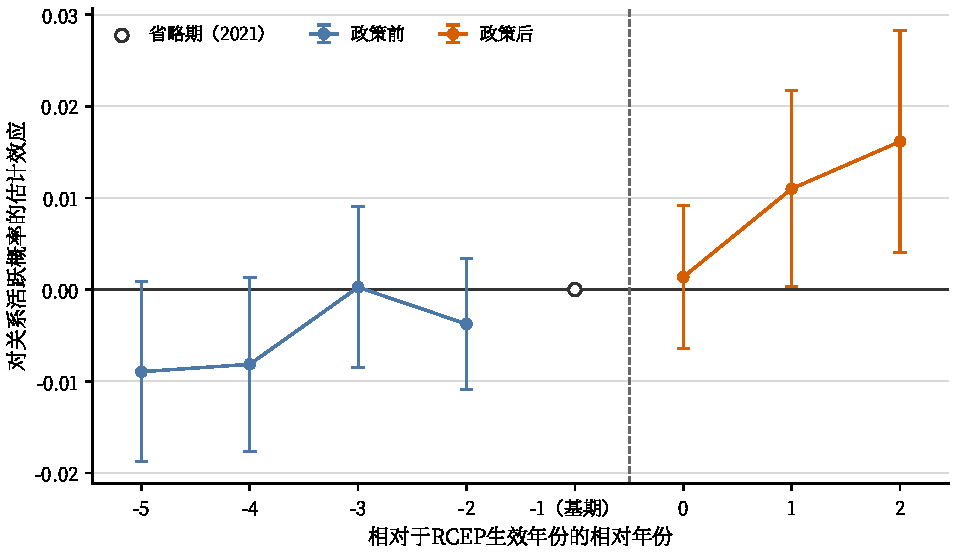
\includegraphics[width=0.92\textwidth]{../results/figures/parallel_trends_standard.pdf}
\caption{\textbf{平行趋势检验：事件研究系数}}
\label{fig:event}
\begin{figurenotes}
\footnotesize
注：点为关系对固定效应和年份固定效应模型中的事件研究系数，误差线为关系对聚类的95\%置信区间。相对年份$-1$（2021年）为省略基期，竖直虚线标记RCEP生效时点。政策前四个系数的等权平均检验在正文中报告。
\end{figurenotes}
\end{figure}

\textbf{安慰剂检验。}本文只保留一个事前设定的时间安慰剂：固定RCEP处理组，将假政策年份设为2019年，并仅使用2017—2021年观测。2019位于可用政策前窗口（2017—2021）的中部，能够在假断点前后各保留观察期；同时它早于2020年11月RCEP签署，避免把签署后的预期反应误当作政策前趋势。该设定检验的是“若在正式签署和生效之前已经存在一个类似断点，模型是否会得到同方向估计”。估计系数为0.007384，关系对聚类标准误为0.003581，$p=0.039217$，样本量为393,925。由于该安慰剂显著，结果并不支持“安慰剂通过”，而是提示真实政策前可能存在时间敏感性或预趋势；选择2019基于窗口位置和制度时点的事前逻辑，而非基于估计显著性。

\textbf{稳健性边界。}上述五个传统规格支持关系对聚类下的正向关联，但不能抵消伙伴国聚类、平行趋势平均检验和2019年时间安慰剂所揭示的识别限制。排除特定伙伴国或疫情年份只能说明样本敏感性，不能单独识别RCEP制度渠道；地理邻近性、区域趋势和协定预期仍可能同时变化。

\textbf{替代解释检验：关税暴露。}表\ref{tab:exclusion}在能够匹配2019年美国关税暴露的企业—伙伴关系样本上报告完整三重交互模型。加入$\text{Post2022}\times\text{TariffExposure}$后，$\text{Post2022}\times\text{RCEP}$系数为$-0.0031$（$p=0.823$）；进一步加入三重交互后，三重交互项系数为0.0471（$p=0.437$）。高关税暴露企业并未表现出统计上更强的RCEP关系变化，因而未发现贸易转移解释的差异性证据。该结果削弱但不能逻辑上排除关税冲突渠道；按伙伴国聚类时三重交互的$p$值为0.661，且匹配样本仅覆盖关系面板约一半企业，结论应作谨慎解释。

\IfFileExists{table6_exclusion.tex}{\begin{table}[htbp]
\centering
\caption{关税暴露替代解释检验}
\label{tab:exclusion}
\small
\begin{tabular}{lrrrr}
\toprule
设定 & 系数 & 标准误 & $p$值 & 观测值 \\\\
\midrule
基准：Post$\times$RCEP & 0.0061 & 0.0065 & 0.346 & 253,184 \\
加入Post$\times$关税暴露 & 0.0063 & 0.0065 & 0.331 & 253,184 \\
三重交互：Post$\times$RCEP$\times$关税暴露 & 0.0471 & 0.0606 & 0.437 & 253,184 \\
\bottomrule
\end{tabular}
\begin{tablenotes}
\footnotesize 注：样本限定为能够匹配2019年美国关税暴露的企业—伙伴关系。所有模型包含企业—伙伴关系对固定效应和年份固定效应，标准误聚类于关系对。美国关税暴露为企业层面的出口加权301/232关税暴露；三重交互项用于检验高关税暴露企业是否具有额外的RCEP关系变化。
\end{tablenotes}
\end{table}}{}

% ═══════════════════════════════════════════════════════════════
% 九、结论
% ═══════════════════════════════════════════════════════════════

\section{结论}

本文利用FactSet Revere全球供应链数据库，追踪中国5,689家上市公司2017—2024年间参与的578,000条供应链关系，以RCEP于2022年1月正式生效为制度时点，在关系对层面构建年度面板。主要发现是一个带有明确识别边界的经验结果，而非对平均因果效应的无条件确认。

第一，在关系对聚类的主规格下，交互项系数为0.013629，标准误0.004046（$p=0.000756$），对应活跃概率约1.36个百分点的正向变化；伙伴国聚类下点估计相同但$ p=0.503$。因此，“显著”是关系对推断下的结果，不应脱离政策暴露层级理解。

第二，将2017—2020年的四个事件研究前置项等权平均后，平均前置效应检验的$p$值为0.180。该结果表明政策前不存在系统性的平均差异，但由于平均检验可能掩盖个别年份偏离，平行趋势仍不能被视为无条件成立。

第三，固定处理组、假政策年份为2019年的时间安慰剂系数为0.007384，标准误0.003581（$p=0.039217$），显示在真实政策前窗口中也能观察到同方向变化。2019的选择基于其位于2017—2021窗口中部、可形成相对平衡的前后观察期且早于2020年签署这一事前制度逻辑，而非依据估计显著性。该安慰剂显著意味着时间敏感性或预趋势不能排除，故不能写成安慰剂通过。

本文的研究存在若干局限。第一，FactSet Revere数据库主要覆盖上市公司和大型企业，中小企业的供应链调整未能纳入分析视野。第二，RCEP生效至今仅三年，关税减让的梯度实施使长期效应尚未充分显现。第三，受限于企业层面海关进出口数据、RCEP原产地证书和企业交易金额数据的可及性，机制检验使用伙伴国—年份层面的政策相关指标，因而只能提供机制一致性证据。第四，地理邻近性与制度效应的不可完全分离，是FTA实证研究中普遍面临的识别挑战。

尽管存在上述局限，本文仍为如何评估区域贸易协定的微观证据提供了边界。关系对层面的正向估计与伙伴国聚类、前置项检验及2019年时间安慰剂并不一致，说明大规模关系数据库不能替代对政策暴露层级和时间识别的严格检验。未来需要产品—国家层面的海关交易、原产地证书和优惠使用数据，才能把制度渠道与同时发生的区域变化区分开来。

% ═══════════════════════════════════════════════════════════════
% 参考文献
% ═══════════════════════════════════════════════════════════════

\begin{thebibliography}{99}

\bibitem{alfaro2023global}
Alfaro, L., \& Chor, D. (2023).
\newblock Global Supply Chains: The Looming ``Great Reallocation''.
\newblock \textit{NBER Working Paper}.

\bibitem{baier2007free}
Baier, S.~L., \& Bergstrand, J.~H. (2007).
\newblock Do free trade agreements actually increase members' international trade?
\newblock \textit{Journal of International Economics}, 71(1), 72--95.

\bibitem{bown2022us}
Bown, C.~P. (2022).
\newblock US-China Trade War Tariffs: An Up-to-Date Chart.
\newblock \textit{Peterson Institute for International Economics}.

\bibitem{crosignani2022pirates}
Crosignani, M., Macchiavelli, M., \& Silva, A.~F. (2022).
\newblock Pirates without borders: The propagation of cyberattacks through firms' supply chains.
\newblock \textit{Journal of Financial Economics}.

\bibitem{difan2022impact}
Di Fan et al. (2022).
\newblock Impact of the US-China trade war on the operating performance of US firms.
\newblock \textit{Journal of Operations Management}.

\bibitem{ding2024trade}
丁浩员等. (2024).
\newblock 贸易政策冲击下的跨国供应链断裂与重构研究.

\bibitem{liu2022rcep}
刘斌, 甄洋. (2022).
\newblock RCEP的贸易效应与规则效应.
\newblock \textit{世界经济研究}.

\bibitem{mahadevan2019can}
Mahadevan, R., \& Nugroho, A. (2019).
\newblock Can the RCEP minimise the harm from the US-China trade war?
\newblock \textit{The World Economy}, 42(11), 3148--3167.

\bibitem{petri2020east}
Petri, P.~A., \& Plummer, M.~G. (2020).
\newblock East Asia decouples from the United States.
\newblock \textit{Peterson Institute Working Paper}.

\bibitem{ping2021rcep}
平力群. (2021).
\newblock RCEP的制度特征及其经济效应.
\newblock \textit{亚太经济}.

\bibitem{shen2011china}
沈铭辉. (2011).
\newblock 中国—东盟自由贸易区: 成就与挑战.
\newblock \textit{当代亚太}.

\bibitem{shen2020rcep}
沈铭辉, 李天国. (2020).
\newblock RCEP: 制度框架、规则特征与区域影响.
\newblock \textit{国际经济评论}.

\bibitem{zhang2021rcep}
张建平, 董亮. (2021).
\newblock RCEP对中国经贸的影响与对策.
\newblock \textit{国际贸易}.

\end{thebibliography}

\end{document}

